\newpage
\section{Self Supervised Methods}
\label{s:ssl}
There's a line of research tackling monocular depth estimation from a self-supervised learning approach.
Well studied geometric relations implicitly constrain depth maps of subsequent frames in videos or in stereo pairs making it suitable to define self-supervised losses for training, i.e. not dependent on ground truth depth maps.
The general idea is simple: given a pair of images geometrically related (e.g. subsequent video frames or a stereo pair), predict the disparity map of one of them and use it to reconstruct the other, the quality of the reconstruction is the target of the optimization.

Before delving into the self supervised works, let's review the main concepts of view synthesis from a disparity map.

Let's consider the pair of images captured by stereo cameras $(\mathbf{I}^{l}, \mathbf{I}^{r})$, respectively captured by a left camera and a right camera, what are their disparity maps $(\mathbf{D}^{l}, \mathbf{D}^{r})$?

Consider a pixel $p$ in the left image $\mathbf{I}^{l}$, this corresponds to a position in the scene 3D space.
This same scene is captured from a different view point by the right camera, the result is the right image $\mathbf{I}^{r}$.
There is a pixel of the right image that corresponds to the pixel $p$ of the left image, meaning that they represent the same location in the scene 3D space and their color is identical.
If we overlap $\mathbf{I}^{l}$ and $\mathbf{I}^{r}$ we can see the displacement between the two pixels, which can be represented as a 2D vector and let's call it $\mathbf{D}^{l}(p)$, so we get:
\[
	\mathbf{I}^{l}(p) = \mathbf{I}^{r}(p + \mathbf{D}^{l}(p))
\]
$\mathbf{D}^{l}(p)$ is the offset to apply to $p$ location in the left image in order to obtain its corresponding location in the right image, hence $\mathbf{D}^{l}$ is a 2D vector field represented by a tensor of shape $H \times W \times 2$.
This was the left disparity map, symmetrically for the right disparity map it holds:
\[
	\mathbf{I}^{r}(p) = \mathbf{I}^{l}(p + \mathbf{D}^{r}(p))
\]
By means of this very symmetry, one disparity map can be written in terms of the other:
\[
\mathbf{D}^{l}(p) = - \mathbf{D}^{r}(p + \mathbf{D}^{l}(p))
\]\[
\mathbf{D}^{r}(p) = - \mathbf{D}^{l}(p + \mathbf{D}^{r}(p))
\]
Now, not every 3D scene location can be visible from all view-points since occlusion can happen.
Thus, disparity maps are not defined at every pixel location.
Another assumption that was made during this discussion is that object appearance is view-point independent, this only holds for Lambertian surfaces and if we do not consider atmospheric effects.
This assumption led to corresponding pixels in different images having the same color.

Assume now that the right image is unknown, given the right disparity map it can be reconstructed in a \textit{differentiable} manner by following the above formulas.
Similarly, for the left image the procedure is the same given the left disparity map.

These formulas make it feasible to reconstruct an image from another given some information about the geometry of the scene, be it in the form of a disparity map or a depth map.
In fact, in the stereo setting, a disparity map can be converted into a depth map and vice-versa \cite{multiview}, although cameras parameters must be known.

Usually stereo-footage from a camera pair is rectified.
Rectifying stereo images means aligning them in such a way that disparity vectors are always horizontal, hence the 2D disparity vector field reduces to a 1D vector field, i.e. represented by a tensor of shape $H \times W$.
This is the setting in which every author that uses stereo video footage find itself in.

%%%%%%%%%%%%%%%%%%%%%%%%%%%%%%%%%%%%%%%%%
%              Garg
%%%%%%%%%%%%%%%%%%%%%%%%%%%%%%%%%%%%%%%%%
\subsection{Garg et al.}
Garg et al. \cite{Garg} rely on having rectified stereo footage with known baseline and camera parameters.
In figure \ref{fig:garg} the training pipeline is illustrated.

% training pipeline
\begin{figure}
	\centering
	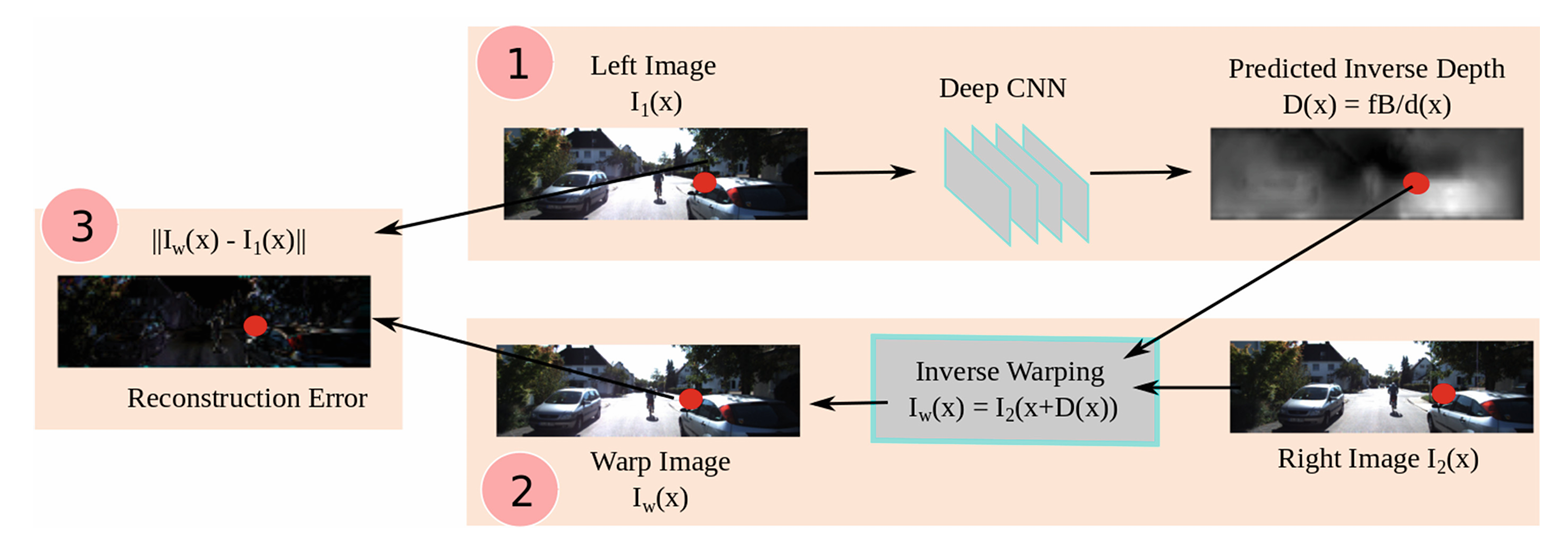
\includegraphics[scale=0.3]{figs/garg}
	\caption{Garg et al. self supervised pipeline \cite{Garg}. \label{fig:garg}}
\end{figure}

Given a stereo pair $\mathbf{I}^{l}, \mathbf{I}^{r}$ they feed $\mathbf{I}^{l}$ to their depth estimation network which returns an estimate of its depth map $\mathbf{Z}^{l}$.
After converting $\mathbf{Z}^{l}$ to a disparity map $\mathbf{D}^{l}$, this can be used to reconstruct the left image using the formula from above: $\hat{\mathbf{I}}^{l} (p) = \mathbf{I}^{r} (p + \mathbf{D}^{l}(p))$, for all pixels $p \in \mathbf{D}^{l}$.
A first order approximation of its gradient is provided through an iterative algorithm, this same procedure represents one of the main limitations of this work since it makes the procedure computationally much more expensive.
The loss to be minimized is the reconstruction error between $\hat{\mathbf{I}}_{l}$ and $\mathbf{I}_{l}$, Garg et al. define it as a mean squared error:
\[
	\mathcal{L}_{rec} = \text{mean}_{p \in \hat{\mathbf{I}}^{l}} \big\| \hat{\mathbf{I}}^{l}(p) - \mathbf{I}^{l}(p) \big\|^{2}
\]
The authors also employ a regularization term that smooths the resulting disparity maps:
\[
	\mathcal{L}_{smooth} = \text{mean}_{p \in \hat{\mathbf{I}}^{l}} \big\| \nabla \mathbf{D}^{l} (p) \big\|^{2}
\]

%%%%%%%%%%%%%%%%%%%%%%%%%%%%%%%%%%%%%%%%%
%              MonoDepth
%%%%%%%%%%%%%%%%%%%%%%%%%%%%%%%%%%%%%%%%%
\subsection{MonoDepth}
Godard et al. \cite{MonoDepth} builds upon the work of Garg et al. \cite{Garg}.
Their method is called MonoDepth.

The limitation of Garg et al. work is now surpassed by employing a simpler sampling procedure for reconstruction that comes from "Spatial Transformer Network" paper \cite{STN}.
This makes the gradient computation exact and cheaper.

If $\mathbf{I}^{l}$ and $\mathbf{D}^{l}$ are given and \textit{stereo baseline and camera parameters are known}, the depth map of $\mathbf{I}^{l}$ can be computed.
Refer to \cite{multiview} for the general case, but in the rectified case is simple trigonometry.
A network for estimating $\mathbf{D}^{l}$ and $\mathbf{D}^{r}$ from $\mathbf{I}^{l}$ is trained.
The estimation of both disparity maps enforces additional consistency.

The loss function to be minimized per image pair is the following:
\[
	\mathcal{L} = \alpha_{ap}(\mathcal{L}_{ap}^{l} + \mathcal{L}_{ap}^{r}) +
		\alpha_{ds}(\mathcal{L}_{ds}^{l} + \mathcal{L}_{ds}^{r}) +
		\alpha_{lr}(\mathcal{L}_{ds}^{l} + \mathcal{L}_{lr}^{r}) 
\]
Where $\alpha_{ap}$, $\alpha_{ds}$, $\alpha_{lr}$ are positive hyperparameters.
While $\mathcal{L}_{ap}$ is the image reconstruction error, $\mathcal{L}_{ds}$ and $\mathcal{L}_{lr}$ are two regularization terms enforcing more geometric consistency in the predicted disparity maps.

\paragraph{Appearance Matching Loss $\mathcal{L}_{ap}$} This is a photometric image reconstruction loss, meaning that penalizes pairs of images appearing too different locally.
How to measure similarity in appearance?
In \cite{SSIM} Wang et al. developed a differentiable similarity index for comparing the appearance of two image patches called \textsc{SSIM}.
In here Godard et al. couple it with the $L1$ loss to account for appearance discrepancies.
\[
	\mathcal{L}_{ap}^{l} = \text{mean}_{p \in \mathbf{I}^{l}}
		\left(
			0.85 \frac{
				1 - \textsc{SSIM} (\mathbf{I}^{l}(p), \hat{\mathbf{I}}^{l}(p))
			}{2} +
			0.15 \big| \mathbf{I}(p)^{l} - \hat{\mathbf{I}}(p)^{l} \big|
		\right)
\]\[
	\mathcal{L}_{ap}^{r} = \text{mean}_{p \in \mathbf{I}^{r}}
		\left(
			0.85 \frac{
				1 - \textsc{SSIM} (\mathbf{I}^{r}(p), \hat{\mathbf{I}}^{r}(p))
			}{2} +
			0.15 \big| \mathbf{I}(p)^{r} - \hat{\mathbf{I}}(p)^{r} \big|
		\right)
\]

\paragraph{Disparity Smoothness Loss $\mathcal{L}_{ds}$} Except for edges and holes in the disparity map, we expect it to be smooth.
How to mathematically express this?
Smoothness (not in the mathematical sense) means a gradient low in magnitude, so that there are not abrupt changes.
The exception is on the edges, which can be loosely characterized as the points with high magnitude image gradient.
By multiplying $\big| \partial \mathbf{D}(p) \big|$ by $e^{- \big| \partial \mathbf{I}(p) \big| }$smoothness is enforced only on the "interior".
Adapting this idea to the fact that images have 3 channels and the gradient operator has two components, the result is:
\[
	\mathcal{L}_{ds}^{l} = \text{mean}_{p \in \mathbf{I}^{l}}
		\left(
			\big| \partial_{x} \mathbf{D}^{l}(p) \big| e^{-\big\| \partial_{x} \mathbf{I}^{l}(p) \big\| } + 
			\big| \partial_{y} \mathbf{D}^{l}(p) \big| e^{-\big\| \partial_{y} \mathbf{I}^{l}(p) \big\| }
		\right)
\]\[
	\mathcal{L}_{ds}^{r} = \text{mean}_{p \in \mathbf{I}^{r}}
		\left(
			\big| \partial_{x} \mathbf{D}^{r}(p) \big| e^{-\big\| \partial_{x} \mathbf{I}^{r}(p) \big\| } + 
			\big| \partial_{y} \mathbf{D}^{r}(p) \big| e^{-\big\| \partial_{y} \mathbf{I}^{r}(p) \big\| }
		\right)
\]

\paragraph{Left-Right Disparity Consistency Loss $\mathcal{L}_{lr}$} This enforces disparity maps to obey above relations.
Notice that even though the losses in the left and right images are perfectly symmetrical, there are image locations in which only one of them makes sense because the other exceeds image boundaries.
Hence, both of them are needed.
\[
	\mathcal{L}_{lr}^{l} = \text{mean}_{p \in \mathbf{I}^{l}}
		\left(
			\big| \mathbf{D}^{l}(p) + \mathbf{D}^{r}(p + \mathbf{D}^{l}(p)) \big|
		\right)
\]\[
	\mathcal{L}_{lr}^{r} = \text{mean}_{p \in \mathbf{I}^{r}}
		\left(
			\big| \mathbf{D}^{r}(p) + \mathbf{D}^{l}(p + \mathbf{D}^{r}(p)) \big|
		\right)
\]
This ends the treatment of this paper.

%%%%%%%%%%%%%%%%%%%%%%%%%%%%%%%%%%%%%%%%%
%              SfMLearner
%%%%%%%%%%%%%%%%%%%%%%%%%%%%%%%%%%%%%%%%%
\subsection{SfMLearner}
Requiring stereo footage for training is a bit of a request, what if simple monocular video footage could be used?
Zhou et al. solve this problem in \cite{SfMLearner} by only asking camera intrinsics to be known.
Their idea is to extract stereo pairs from a monocular video footage.
In fact, if the scene is static and subsequent frames are taken from different angles then these frames can be thought as a stereo pair.
The next step is to estimate the unknown camera transformation between the two frames.
The figure \ref{fig:sfmlearner} shows the general procedure called SfMLearner (Structure from Motion Learner).

% training pipeline
\begin{figure}
	\centering
	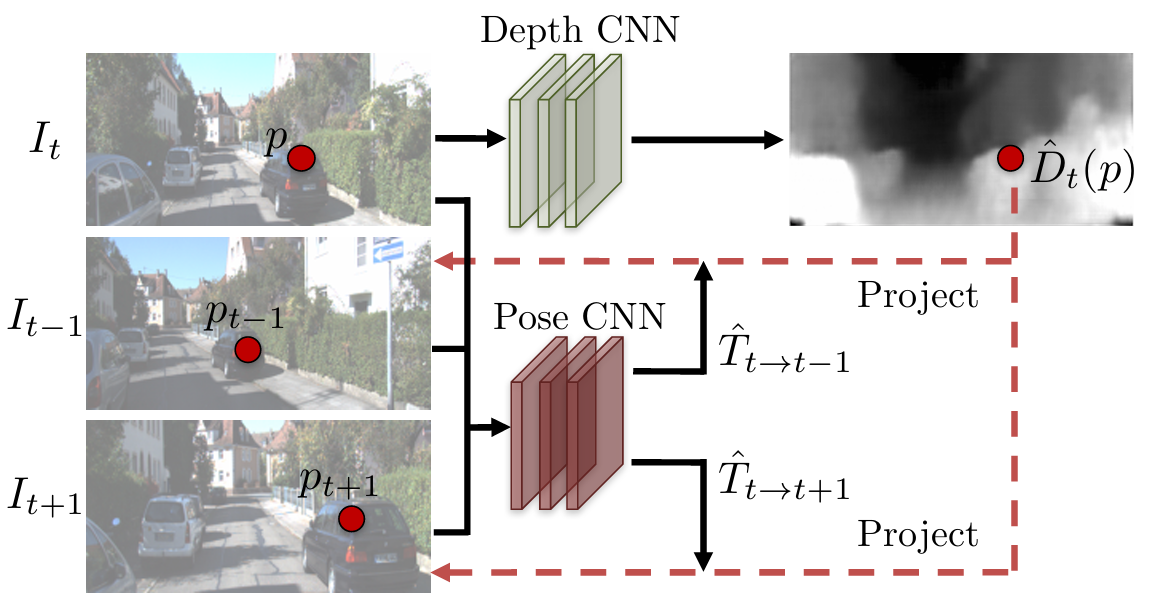
\includegraphics[scale=0.3]{figs/sfmlearner}
	\caption{Zhou et al. self supervised pipeline \cite{SfMLearner} that uses monocular video footage. \label{fig:sfmlearner}}
\end{figure}

Starting simple: if an image $\mathbf{I}$, its depth map $\mathbf{Z}$ and the camera intrinsics matrix $\mathbf{K}$ are given, then each pixel location $p$ can be \textit{differentiably} back-projected to its scene 3D space location $\mathbf{x}$ (refer to \cite{multiview} as usual).
$\mathbf{x}$ is expressed w.r.t. the camera reference frame.
If the camera is moved through a rigid transformation $\mathcal{T}$ (i.e. translation and rotation) then $\mathcal{T}^{-1} (\mathbf{x})$ are the coordinates w.r.t. the new reference frame.
The updated $\mathbf{x}$ can now be projected to the new image plane.
This procedure can be used to reconstruct one image from the other, given the depth map of one of them.
Zhou et al. call "\textit{target} frame" the one to reconstruct and "\textit{source} frame" the one used for reconstruction.
The depth map of the target frame is used for its reconstruction.
The authors use three subsequent video frames $\mathbf{I}_{t-1}$, $\mathbf{I}_{t}$ and $\mathbf{I}_{t+1}$.
The middle frame is the target frame and the other two are source frames.
A neural network is used for estimating the depth map $\mathbf{Z}$ of $\mathbf{I}_{t}$ and another for estimating the ego-motion between two subsequent frames, e.g. the transformation $\mathcal{T}_{t \rightarrow t+1}$ that the camera goes through to pass from the setting at time $t$ to the setting at time $t+1$.
The transformation $\mathcal{T}_{t \rightarrow t+1}$ is predicted by means of its parametrization $(\theta_{x}, \theta_{y}, \theta_{z}, t_{x}, t_{y}, t_{z})$, hence only 6 numbers are required.

One important consideration: why are three frames used and not just two and, why is the middle one targeted?
Usually, video footage is recorded \textit{moving forward}, as it is the case for the KITTI dataset on which Zhou et al. train their model.
This implies that the camera pose estimation network would have got a strong bias if only \textit{two} subsequent frames were considered.
Considering \textit{three} of them and targeting the middle one balances the situation for it learns to reconstruct both moving forward and moving backward.
A theoretical alternative might have been to estimate the pose between two subsequent frames one from the other symmetrically.

For what concerns the loss function here used, less specific choices have been made with respect to MonoDepth.
The loss is defined as:
\[
	\mathcal{L} = \mathcal{L}_{vs}(\hat{\mathbf{I}}, \mathbf{I}) + \mathcal{L}_{smooth}(\mathbf{D}) + \mathcal{L}_{reg}
\]
Where $\mathcal{L}_{vs}$ is the view synthesis loss, which is simply implemented as an $L1$ loss between the source frame and its synthesis; $\mathcal{L}_{smooth}$ is the $L1$ norm of the second-order gradients for the predicted depth maps and $\mathcal{L}_{reg}$ is a regularization term, actually there is a last ingredient I omitted that I am to introduce.
As should be clear by now, image reconstruction from different views is heavily based on assumptions that don't often hold in the real world.
Zhou et al. thought of weighting every pixel in the view synthesis reconstruction loss with a zero to one value $\hat{\mathbf{E}}(p)$ that represents the success probability of the view-synthesis process in $p$.
So that:
\[
	\mathcal{L}_{vs} = \text{mean}_{p \in \mathbf{I}}
		\left(
			\hat{\mathbf{E}}(p) \big| \mathbf{I}(p) - \hat{\mathbf{I}}(p) \big|
		\right)
\]
$\hat{\mathbf{E}}(p)$ is computed within the same pipeline that predicts the camera poses.
This neural network encodes subsequent frames and then: one little network regresses camera transformation free parameters and a decoder compute this confidence score $\hat{\mathbf{E}}$ pixel-wise and at multiple scales.
Depth maps are computed at multiple scales by using a DispNet \cite{DispNet} architecture.
$\mathcal{L}_{reg}$ regularizes $\hat{\mathbf{E}}$ discouraging it to be the trivial zero solution.
Although, in a more recent version of the model, the authors claim that by using data-augmentation they managed to get rid of this regularization term.

%%%%%%%%%%%%%%%%%%%%%%%%%%%%%%%%%%%%%%%%%
%              Vid2Depth
%%%%%%%%%%%%%%%%%%%%%%%%%%%%%%%%%%%%%%%%%
\subsection{vid2depth}
Mahjourian et al. develop vid2depth \cite{vid2depth}, a method that directly improves SfMLearner by explicitly working in the 3D space geometry.
The idea is to work with point clouds rather than depth maps, an image from the paper can be found in figure \ref{fig:vid2depth}.

% training pipeline
\begin{figure}
	\centering
	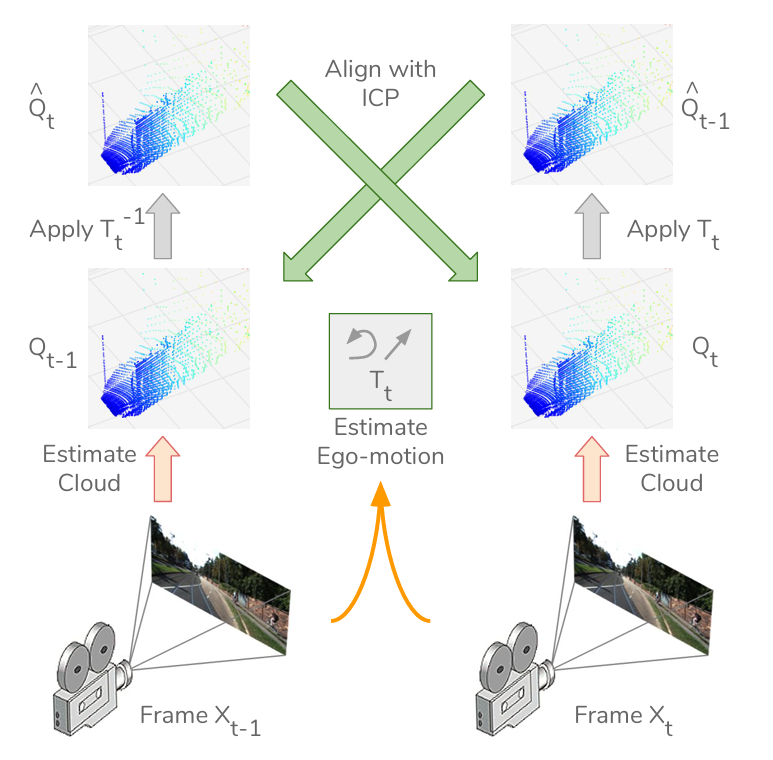
\includegraphics[scale=0.3]{figs/vid2depth}
	\caption{Mahjourian et al. self supervised training pipeline \cite{vid2depth}. \label{fig:vid2depth}}
\end{figure}

The authors' idea is to explicitly constrain consistency on 3D point clouds.
Given two subsequent video frames $\mathbf{I}$ and $\mathbf{J}$, the ego-motion $\mathcal{T} = f_{pose}(\mathbf{I}, \mathbf{J})$ and depth maps of both frames $\mathbf{D}^{\mathbf{I}} = f_{depth}(\mathbf{I}), \mathbf{D}^{\mathbf{J}} = f_{depth}(\mathbf{J})$ are estimated.
Thanks to the (supposedly known) camera intrinsics matrix $\mathbf{K}$, depth maps can be converted into 3D point clouds $\mathbf{Q}_{\mathbf{I}}, \mathbf{Q}_{\mathbf{J}}$.
If $\mathcal{T}$ is the transformation of the camera from $\mathbf{I}$ to $\mathbf{J}$, then $\mathcal{T} ( \mathbf{Q}_{\mathbf{J}} )$ is $\mathbf{Q}_{\mathbf{J}}$ looked from the $\mathbf{I}$ camera and, in theory, it should be identical to $\mathbf{Q}_{\mathbf{I}}$.
A measure of the misalignment of the two point clouds is not defined and, even if it was, it would probably be not differentiable.
Mahjourian et al. solution is to use some registration algorithm for estimating what's the best alignment of the two point clouds by rigid transforming $\mathbf{Q}_{\mathbf{J}}$ to match $\mathbf{Q}_{\mathbf{I}}$ and what the residual error would be.
Then, push $\mathcal{T}$ to match that best rigid transform and push 3D points pair chosen by the algorithm to get more close after the transformation.
They use Iterative Closest Point (ICP) algorithm, which is a registration algorithm that basically tells which points correspond between the two clouds and what's the overall best rigid transformation that one point cloud (following the previous discussion this would be $\mathbf{Q}_{\mathbf{J}}$) should undergo to match the other one($\mathbf{Q}_{\mathbf{I}}$).
"Best" here means that it minimizes the mean distance between the selected point pairs.
So, ICT returns this estimated transform $\hat{\mathcal{T}}$, which can be expressed using its 6 free parameters $(\hat{\theta}_{x}, \hat{\theta}_{y}, \hat{\theta}_{z}, \hat{t}_{x}, \hat{t}_{y}, \hat{t}_{z})$, and directly compared with the ones from the pose-network.
The resulting loss looks like this:
\[
	\big| \hat{\theta}_{x} - \theta_{x} \big| +
	\big| \hat{\theta}_{y} - \theta_{y} \big| +
	\big| \hat{\theta}_{z} - \theta_{z} \big| +
	\big| \hat{t}_{x} - t_{x} \big| +
	\big| \hat{t}_{y} - t_{y} \big| +
	\big| \hat{t}_{z} - t_{z} \big|
\]
This sorts out the pose network optimization, for the depth network it is instead optimized:
\[
	\sum_{p_{\mathbf{I}} \, \text{matches} \, p_{\mathbf{J}}} \big| p_{\mathbf{I}} - \mathcal{T} (p_{\mathbf{J}}) \big|
\]

%%%%%%%%%%%%%%%%%%%%%%%%%%%%%%%%%%%%%%%%%
%              MonoDepth2
%%%%%%%%%%%%%%%%%%%%%%%%%%%%%%%%%%%%%%%%%
\subsection{MonoDepth2}
Quoting Godard et al. from the abstract of \cite{MonoDepth2}: \textit{"We show that a surprisingly simple model, and associated design choices, lead to superior predictions"}.
In this work they take MonoDepth \cite{MonoDepth} and improve it with clever small tricks without changing the spirit of the method, although adapting it to be trained also on monocular video footage like in \cite{SfMLearner}.
In fact, in MonoDepth images were labeled as "left" or "right", in here the general distinction is between "source" and "target".

In their edge-aware smoothness loss, the authors substitute $\mathbf{D}$ with its mean normalized value $\mathbf{D} / \text{mean} \mathbf{D}$ to discourage shrinking of the estimated disparity map.

Next they improve the reconstruction error loss: if $\mathbf{I}_{target}$ is reconstructed from $\mathbf{I}_{source, 1}$ obtaining $\hat{\mathbf{I}}_{target, 1}$ and reconstructed from $\mathbf{I}_{source, 2}$ obtaining $\hat{\mathbf{I}}_{target, 2}$, previously the two reconstruction losses were averaged like this:
\[
	\text{mean}_{p \in \mathbf{I}_{target}} \frac{1}{2}(\mathcal{L}_{rec}(\hat{\mathbf{I}}_{target, 1}(p), \mathbf{I}_{target}(p)) + \mathcal{L}_{rec}(\hat{\mathbf{I}}_{target, 2}(p), \mathbf{I}_{target}(p)))
\]
Though, it is better to minimize the smallest term between the two because the largest is likely linked to phenomenons like occlusion or out-of-view pixel and nothing can be done about it.
Usually, if something is occluded in a view, it is not in the other!
Same thing for out-of-view pixels.
So it is now minimized
\[
	\text{mean}_{p \in \mathbf{I}_{target}} \text{min} \{ \mathcal{L}_{rec}(\hat{\mathbf{I}}_{target, 1}(p), \, \mathbf{I}_{target}(p)), \, \mathcal{L}_{rec}(\hat{\mathbf{I}}_{target, 2}(p), \mathbf{I}_{target}(p)) \}
\]
In here $\mathcal{L}_{rec}$ represents the photometric error computed pixel-wise.
Godard et al. use the same error as in MonoDepth through the SSIM and L1 loss.

Another clever improvement Godard et al. make is to apply an auto-masking procedure for stationary pixels.
Static pixels can correspond to a static camera or to objects moving at the same velocity of the camera.
If a pixel $p$ is such that $\mathcal{L}_{rec}(\mathbf{I}_{target}(p), \mathbf{I}_{source}(p))$ is "low", then there are three likely alternatives:
\begin{enumerate}
\item the camera is not moving and that pixel corresponds to a static object
\item the camera is moving and that pixel corresponds to an object moving in the same direction and speed of the camera
\item that pixel corresponds to a low texture area, hence, independently of the dynamics of the scene, it is similar across adjacent frames.
\end{enumerate}
The heuristic is to mask out pixels that have this "low" comparison error.
Godard et al. exclude pixels with comparison error smaller than the reconstruction error:
\[
	\text{Consider only } p \in \mathbf{I}_{target} \text{ such that: }
\]\[
	\mathcal{L}_{rec}(\mathbf{I}_{target}(p), \mathbf{I}_{source}(p))
		\leq
	\mathcal{L}_{rec}(\mathbf{I}_{target}(p), \hat{\mathbf{I}}_{target}(p))
\]
If multiple source images are used for reconstruction, take the minimum of both members with respect to the sources.

Their observations and tricks continue on the architectural side.
For instance, they up-sample the lower resolution depth maps returned by their multiscale network instead of decreasing the resolution of the ground truth data during training.
They also apply reflection padding to input images to decrease border artifacts, as opposed to zero-padding.

%%%%%%%%%%%%%%%%%%%%%%%%%%%%%%%%%%%%%%%%%
%              struct2depth
%%%%%%%%%%%%%%%%%%%%%%%%%%%%%%%%%%%%%%%%%
\subsection{struct2depth}
What's the next step? To weaken assumptions.
One very limiting assumption was that video footage scenes were static, i.e. nothing moves.
In \cite{struct2depth} Casser et al. try to include the motion of the objects into their framework, which they call struct2depth (see figure \ref{fig:struct2depth}).
They are not the first to model dynamic scenes for improving depth estimation from subsequent frames, but they are the first that model individual objects movements rather than using 2D or 3D optical flow.

% architecture
\begin{figure}
	\centering
	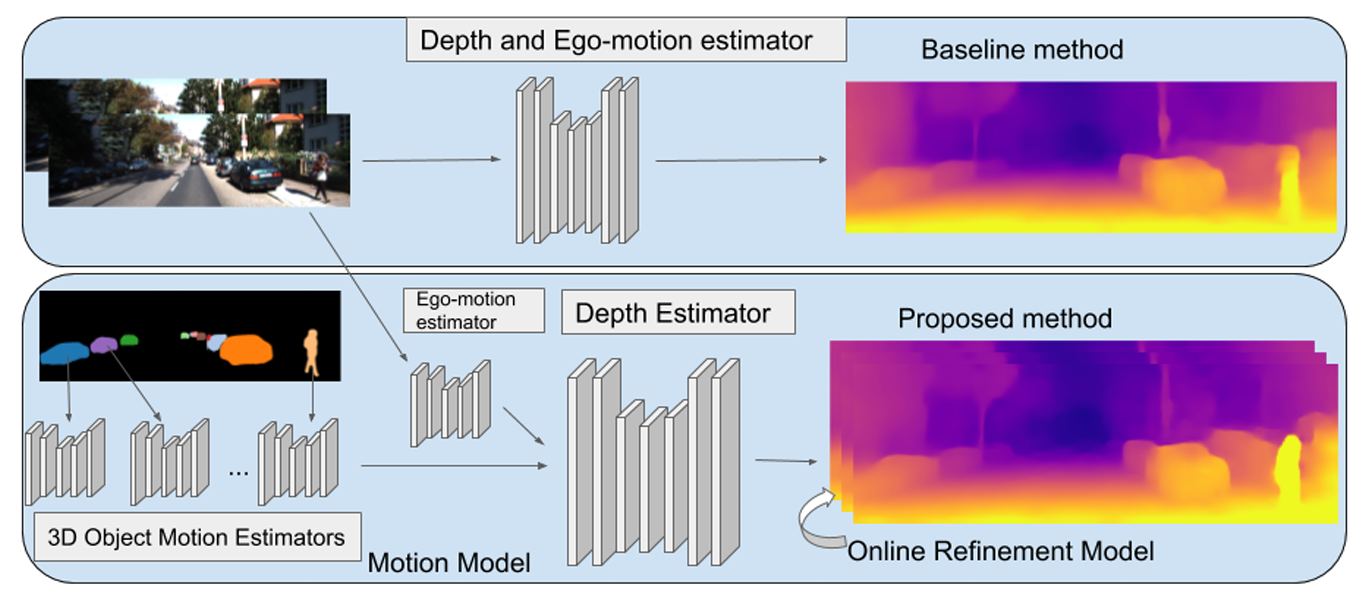
\includegraphics[scale=0.3]{figs/struct2depth}
	\caption{Casser et al. struct2depth \cite{struct2depth} model. \label{fig:struct2depth}}
\end{figure}

As always let's first simplify the approach.
Consider an object which appears in subsequent frames, if images are masked so that only the object is visible, the relative transformation of the camera w.r.t. it can be estimated.
Thanks to that it might be reconstructed the object appearance in one frame from its appearance in the other.
More precisely, consider $\mathbf{I}_{0}$ and $\mathbf{I}_{1}$ are the two frames and the object masks are $\mathbf{O}_{0}$ and $\mathbf{O}_{1}$ (which can be computed by means of a given instance-aligned segmentation model $f_{segment}$).
The relative camera transformation $\mathcal{T}$ can be estimated as $f_{pose}(\mathbf{I}_{0} \odot \mathbf{O}_{0}, \, \mathbf{I}_{1} \odot \mathbf{O}_{1})$, with $\odot$ representing pixel-wise multiplication.
For reconstruction purpose, a depth map is estimated from the first image: $\mathbf{Z}_{0} = f_{depth}(\mathbf{I}_{0})$.
Now $\mathbf{Z}_{0}$ gives the depth of the object in the nonzero pixels of its mask $\mathbf{O}_{0}$.
The same reconstruction of the previous methods is applied.
The only difference is not all target image $\mathbf{I}_{1}$ pixels are filled, but just the ones corresponding to the object, i.e. the non-masked pixels from $\mathbf{O}_{1}$.

The way the authors put all of this together in an actual procedure is a bit more complicated, here only a general overview is reported.
They consider three frames and target the middle one for the reconstruction by first applying the illustrated procedure on the background mask and actually reconstructing the whole image without considering moving objects artifacts.
Then they segment the objects in this reconstruction and apply the procedure again to them.
In this way they separate objects motion from ego-motion and for this purpose they use two different pose networks.
For technical details and considerations they follow along Godard et al. and their MonoDepth2 \cite{MonoDepth2}.

One important contribution of Casser et al. work is to include constraints on object sizes in regressing the depth.
This is very clever and solves a problem encountered in MonoDepth2 which was there tackled using stereo data.
If I am in a car capturing video footage and in front of me there is a car moving at the same speed, the model will assign to it "infinite" depth, like it were a very far background detail like the sky is.
For solving this, Casser et al. guess the depth of the objects based on their size (i.e. area) and class (car, tree, person, ...) and constrain also the depth model to have a similar guess.

There are other things that could be added, but I think this is sufficient to grasp the general concept.

%%%%%%%%%%%%%%%%%%%%%%%%%%%%%%%%%%%%%%%%%
%              struct2depth
%%%%%%%%%%%%%%%%%%%%%%%%%%%%%%%%%%%%%%%%%
\subsection{FeatDepth}
Why need I compare images using their appearance and not some higher representation of them?
No reasons, in fact Shu et al. \cite{FeatDepth} propose to compare reconstructed images based on their feature maps.

% training pipeline
\begin{figure}
	\centering
	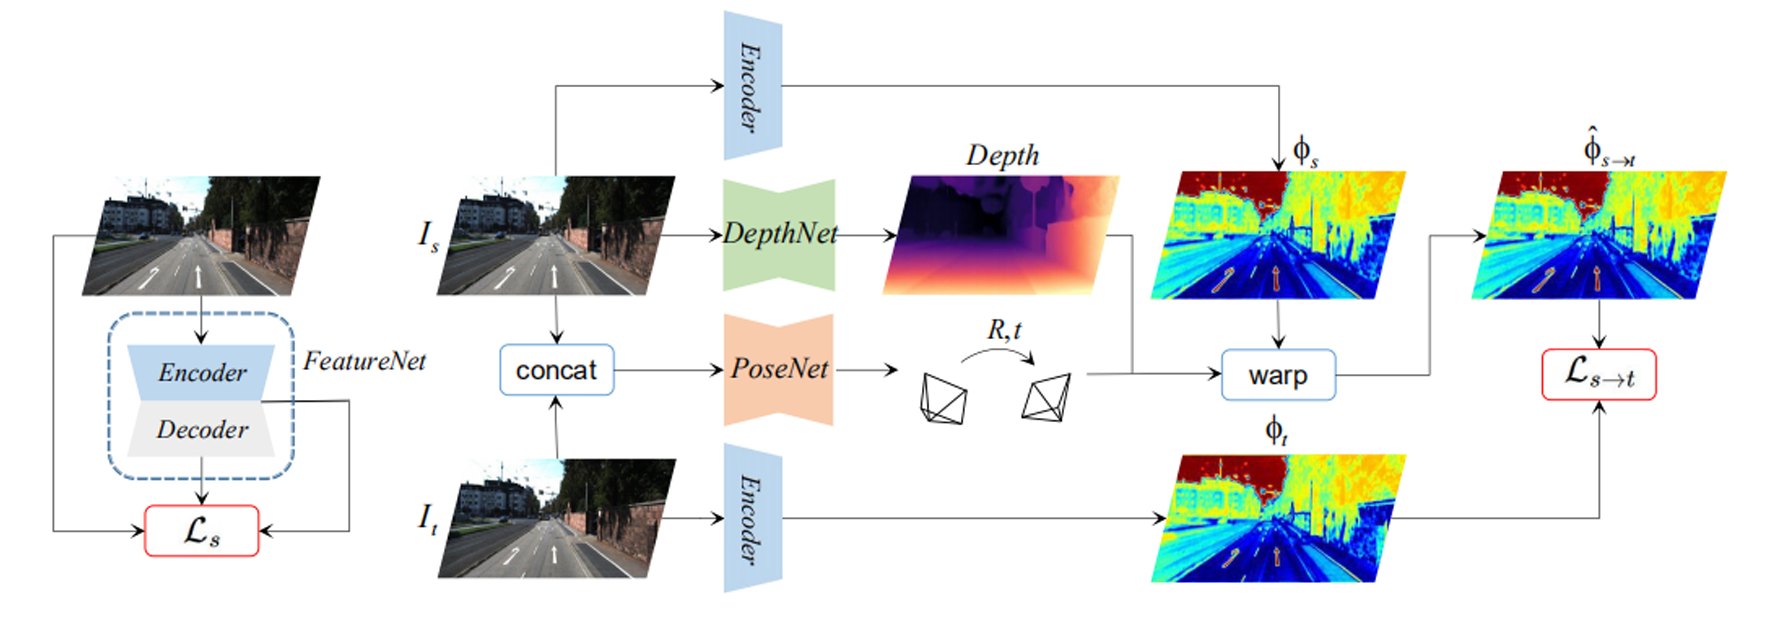
\includegraphics[scale=0.3]{figs/featdepth}
	\caption{Shu et al. FeatDepth \cite{FeatDepth} pipeline. Note that the image is taken from the paper and uses a different notation. \label{fig:featdepth}}
\end{figure}

They argue that correct depth and pose are sufficient but not necessary for small photometric error.
The cause of this is texture-less regions which produce low photometric error even with wrong depth and pose estimates.
The authors' idea is then to use some higher representation of the image encouraging it to be discriminative also where the image is not.
For achieving this, Shu et al. employ three networks: DepthNet and PoseNet, as in the previous works, and FeatureNet which is an encoder based on ResNet-50 \cite{ResNet}.
If $\mathbf{F}$ is the deep multi-channel feature map of the image to reconstruct $\mathbf{I}$ and $\mathbf{F}_{rec}$ the one of the reconstructed image $\mathbf{I}_{rec}$, then the following losses are used:
\[
	\mathcal{L}_{rec} = \text{mean}_{p \in \mathbf{F}} \big\| \mathbf{F}(p) - \mathbf{F}_{rec}(p) \big\|
\] \[
	\mathcal{L}_{dis} = - \text{mean}_{p \in \mathbf{F}} \big\| \nabla^{1} \mathbf{F}(p) \big\|
\] \[
	\mathcal{L}_{cvt} = \text{mean}_{p \in \mathbf{F}} \big\| \nabla^{2} \mathbf{F}(p) \big\|
\]
$\mathcal{L}_{rec}$ is the reconstruction error measured in the feature space.
$\mathcal{L}_{dis}$ encourages the learned feature maps to have gradients, making also texture-less regions well characterized.
Lastly, $\mathcal{L}_{cvt}$ is a regularization term favouring the convergence of the method.

The architecture of FeatDepth is improved in GCNDepth \cite{GCNDepth} by other authors.
They use a Graph Convolutional Network (GCN) for mapping intermediate decoder feature maps to depth maps, managing to reduce the size of their model of 40\% w.r.t. FeatDepth.